\documentclass[11pt,a4paper,oneside]{book}

% ============================================
% PACKAGES
% ============================================
\usepackage[utf8]{inputenc}
\usepackage[T1]{fontenc}
\usepackage[english]{babel}
\usepackage{geometry}
\usepackage{titlesec}
\usepackage{fancyhdr}
\usepackage{graphicx}
\usepackage{xcolor}
\usepackage{tcolorbox}
\usepackage{tikz}
\usepackage{pgfplots}
\usepackage{listings}
\usepackage{hyperref}
\usepackage{tabularx}
\usepackage{booktabs}
\usepackage{enumitem}
\usepackage{fontawesome5}
\usepackage{multicol}
\usepackage{amsmath}
\usepackage{array}

% ============================================
% DOCUMENT GEOMETRY
% ============================================
\geometry{
    a4paper,
    left=2.5cm,
    right=2.5cm,
    top=2.5cm,
    bottom=3cm,
    headheight=15pt
}

% ============================================
% COLOR DEFINITIONS
% ============================================
\definecolor{appwritepink}{RGB}{253,54,110}
\definecolor{appwritedark}{RGB}{25,25,28}
\definecolor{primarynavy}{RGB}{20,40,80}
\definecolor{accentteal}{RGB}{0,150,136}
\definecolor{accentblue}{RGB}{33,150,243}
\definecolor{darkgray}{RGB}{50,50,50}
\definecolor{lightgray}{RGB}{240,240,240}
\definecolor{codebackground}{RGB}{245,245,250}

% ============================================
% TIKZ LIBRARIES
% ============================================
\usetikzlibrary{shapes,arrows,positioning,shadows,calc}
\pgfplotsset{compat=1.18}

% ============================================
% HYPERREF SETUP
% ============================================
\hypersetup{
    colorlinks=true,
    linkcolor=primarynavy,
    filecolor=appwritepink,
    urlcolor=appwritepink,
    citecolor=primarynavy,
    pdftitle={Appwrite Complete Guide for Mobile Development},
    pdfauthor={Mausam Kar},
    pdfsubject={Backend as a Service},
    pdfkeywords={Appwrite, BaaS, Mobile Development, Backend}
}

% ============================================
% CHAPTER & SECTION STYLING
% ============================================
\titleformat{\chapter}[block]
  {\normalfont\huge\bfseries\color{appwritedark}}
  {\colorbox{appwritepink}{\parbox{1.5cm}{\centering\textcolor{white}{\fontsize{40}{48}\selectfont\thechapter}}}}
  {1em}
  {\Huge}
  [\vspace{2ex}\titlerule]

\titleformat{\section}
  {\normalfont\Large\bfseries\color{appwritedark}}
  {\thesection}
  {1em}
  {}
  [\vspace{0.5ex}{\color{appwritepink}\titlerule[1pt]}]

\titleformat{\subsection}
  {\normalfont\large\bfseries\color{appwritepink}}
  {\thesubsection}
  {1em}
  {}

% ============================================
% HEADER & FOOTER
% ============================================
\pagestyle{fancy}
\fancyhf{}
\fancyhead[L]{\nouppercase{\leftmark}}
\fancyhead[R]{\textcolor{appwritepink}{\textbf{Appwrite Guide}}}
\fancyfoot[C]{\thepage}
\renewcommand{\headrulewidth}{0.5pt}
\renewcommand{\footrulewidth}{0pt}

% ============================================
% COLORED BOXES
% ============================================
\tcbuselibrary{skins,breakable}

\newtcolorbox{definitionbox}{
    colback=accentteal!5,
    colframe=accentteal,
    fonttitle=\bfseries,
    title=Definition,
    boxrule=1pt,
    arc=3pt,
    breakable
}

\newtcolorbox{keypoint}{
    colback=appwritepink!10,
    colframe=appwritepink,
    fonttitle=\bfseries,
    title=Key Point,
    boxrule=1pt,
    arc=3pt,
    breakable
}

\newtcolorbox{notebox}{
    colback=accentblue!5,
    colframe=accentblue,
    fonttitle=\bfseries,
    title=Note,
    boxrule=1pt,
    arc=3pt,
    breakable
}

\newtcolorbox{warningbox}{
    colback=orange!10,
    colframe=orange,
    fonttitle=\bfseries,
    title=Warning,
    boxrule=1pt,
    arc=3pt,
    breakable
}

% ============================================
% CODE LISTING STYLE
% ============================================
\lstset{
    backgroundcolor=\color{codebackground},
    basicstyle=\ttfamily\small,
    keywordstyle=\color{appwritepink}\bfseries,
    stringstyle=\color{accentteal},
    commentstyle=\color{gray}\itshape,
    numberstyle=\tiny\color{gray},
    numbers=left,
    breaklines=true,
    frame=single,
    rulecolor=\color{lightgray},
    tabsize=2,
    captionpos=b,
    showstringspaces=false
}

% ============================================
% DOCUMENT BEGIN
% ============================================
\begin{document}

% ============================================
% TITLE PAGE
% ============================================
\begin{titlepage}

\begin{tikzpicture}[remember picture,overlay]
    % Background
    \fill[appwritedark] (current page.south west) rectangle (current page.north east);
    
    % Top accent
    \fill[appwritepink] (current page.north west) rectangle ([yshift=-3cm]current page.north east);
    
    % Bottom accent
    \fill[accentteal] (current page.south west) rectangle ([yshift=2.5cm]current page.south east);
    
    % Decorative elements
    \foreach \i in {1,...,6}{
        \fill[white,opacity=0.05] ([xshift=\i cm, yshift=-\i cm]current page.north east) circle (2.5cm);
    }
    
    % Title
    \node[text width=13cm,align=center] at (current page.center) {
        {\Huge\bfseries\color{white} APPWRITE}\\[0.5cm]
        {\LARGE\color{appwritepink} Complete Guide for Mobile Development}\\[0.8cm]
        {\large\color{lightgray} Backend-as-a-Service Platform}\\[3cm]
        {\Large\color{white} Master Backend Development}\\[0.3cm]
        {\large\color{lightgray} Authentication • Databases • Storage • Functions • Realtime}\\[4cm]
        {\LARGE\bfseries\color{accentteal} Mausam Kar}\\[0.3cm]
        {\large\color{white} Full-Stack Developer}
    };
    
    % Version
    \node[fill=appwritepink,rounded corners,text=white,font=\bfseries] at ([yshift=3cm]current page.south) {Comprehensive Documentation | 2024};
\end{tikzpicture}
\end{titlepage}

\frontmatter
\tableofcontents

\mainmatter

% ============================================
% CHAPTER 1: INTRODUCTION
% ============================================
\chapter{Introduction to Appwrite}

\section{What is Appwrite?}

\begin{definitionbox}
\textbf{Appwrite} is an open-source, self-hosted Backend-as-a-Service (BaaS) platform that provides developers with a set of APIs and tools to build secure and scalable applications faster. It eliminates the need to build backend infrastructure from scratch.
\end{definitionbox}

Appwrite provides ready-to-use backend services including:

\begin{itemize}[leftmargin=2cm]
    \item[\faLock] \textbf{Authentication} - User management and secure login
    \item[\faDatabase] \textbf{Databases} - NoSQL document databases
    \item[\faCloud] \textbf{Storage} - File storage and CDN
    \item[\faCode] \textbf{Functions} - Serverless cloud functions
    \item[\faBolt] \textbf{Realtime} - WebSocket connections
    \item[\faGlobe] \textbf{Localization} - Multi-language support
\end{itemize}

\section{Why Appwrite for Mobile Apps?}

\begin{table}[h]
\centering
\begin{tabularx}{\textwidth}{l X}
\toprule
\textbf{Advantage} & \textbf{Benefit} \\
\midrule
Cross-Platform SDKs & Native support for iOS, Android, Flutter, React Native \\
Secure by Default & Built-in security features and encryption \\
Scalable Architecture & Auto-scaling and load balancing \\
Developer Friendly & Clean APIs and comprehensive documentation \\
Open Source & Free, transparent, and community-driven \\
Self-Hosted Option & Full control over your data \\
\bottomrule
\end{tabularx}
\caption{Appwrite Advantages for Mobile Development}
\end{table}

\section{Key Features}

\begin{keypoint}
Appwrite provides over \textbf{18+ products and services} including:
\begin{multicols}{2}
\begin{itemize}
    \item Account Management
    \item OAuth2 Providers
    \item Team Collaboration
    \item Database Collections
    \item File Storage
    \item Cloud Functions
    \item Webhooks
    \item Realtime Updates
    \item Health Monitoring
    \item Locale Detection
    \item Avatar Generation
    \item Email/SMS
\end{itemize}
\end{multicols}
\end{keypoint}

% ============================================
% CHAPTER 2: ARCHITECTURE
% ============================================
\chapter{Appwrite Architecture}

\section{System Architecture}

\begin{figure}[h]
\centering
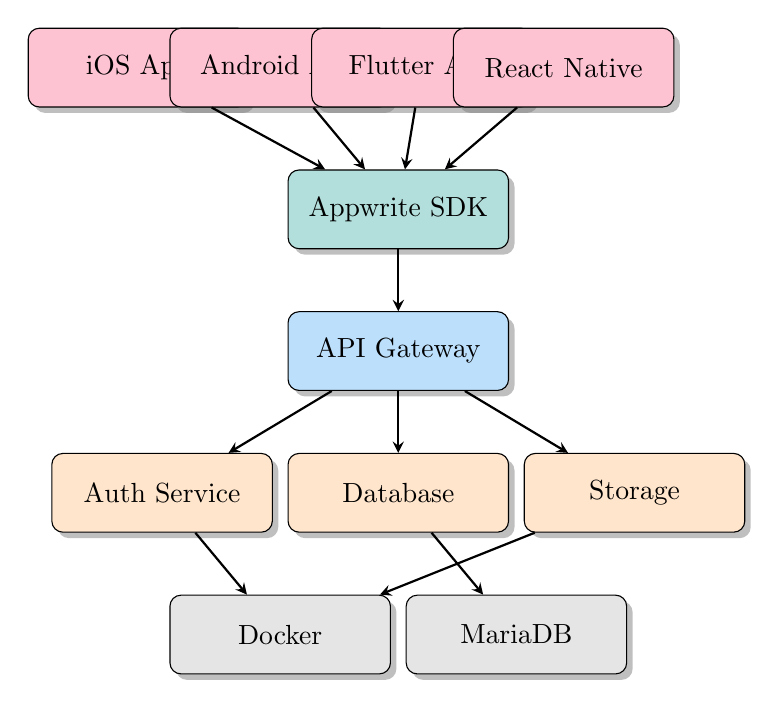
\begin{tikzpicture}[
    node distance=1.8cm,
    box/.style={rectangle, rounded corners, minimum width=2.8cm, minimum height=1cm, text centered, draw=black, fill=blue!20, drop shadow},
    arrow/.style={->, >=stealth, thick}
]

% Mobile Apps Layer
\node[box, fill=appwritepink!30] (ios) at (0,0) {iOS App};
\node[box, fill=appwritepink!30, right of=ios] (android) {Android App};
\node[box, fill=appwritepink!30, right of=android] (flutter) {Flutter App};
\node[box, fill=appwritepink!30, right of=flutter] (rn) {React Native};

% SDK Layer
\node[box, fill=accentteal!30, below of=android, xshift=1.5cm] (sdk) {Appwrite SDK};

% API Gateway
\node[box, fill=accentblue!30, below of=sdk] (gateway) {API Gateway};

% Services Layer
\node[box, fill=orange!20, below of=gateway, xshift=-3cm] (auth) {Auth Service};
\node[box, fill=orange!20, below of=gateway] (db) {Database};
\node[box, fill=orange!20, below of=gateway, xshift=3cm] (storage) {Storage};

% Infrastructure
\node[box, fill=gray!20, below of=db, xshift=-1.5cm] (docker) {Docker};
\node[box, fill=gray!20, below of=db, xshift=1.5cm] (mariadb) {MariaDB};

% Arrows
\draw[arrow] (ios) -- (sdk);
\draw[arrow] (android) -- (sdk);
\draw[arrow] (flutter) -- (sdk);
\draw[arrow] (rn) -- (sdk);
\draw[arrow] (sdk) -- (gateway);
\draw[arrow] (gateway) -- (auth);
\draw[arrow] (gateway) -- (db);
\draw[arrow] (gateway) -- (storage);
\draw[arrow] (auth) -- (docker);
\draw[arrow] (db) -- (mariadb);
\draw[arrow] (storage) -- (docker);

\end{tikzpicture}
\caption{Appwrite System Architecture}
\end{figure}

\section{Core Components}

\subsection{API Gateway}
Central entry point that routes requests to appropriate services, handles authentication, and enforces security policies.

\subsection{Services Layer}
Individual microservices for authentication, database, storage, functions, and more.

\subsection{Docker Infrastructure}
Containerized deployment for easy scaling and management.

% ============================================
% CHAPTER 3: AUTHENTICATION
% ============================================
\chapter{Authentication \& User Management}

\section{Authentication Methods}

Appwrite supports multiple authentication methods:

\begin{table}[h]
\centering
\begin{tabularx}{\textwidth}{l X c}
\toprule
\textbf{Method} & \textbf{Description} & \textbf{Use Case} \\
\midrule
Email/Password & Traditional email and password & Standard apps \\
Magic URL & Passwordless email link & User convenience \\
Phone (SMS) & OTP via SMS & Mobile-first apps \\
Anonymous & Temporary anonymous sessions & Guest access \\
OAuth2 & 30+ providers (Google, Facebook, etc.) & Social login \\
JWT & Custom token authentication & Enterprise apps \\
\bottomrule
\end{tabularx}
\caption{Appwrite Authentication Methods}
\end{table}

\section{OAuth2 Implementation}

\begin{lstlisting}[language=JavaScript, caption=Google OAuth Implementation]
import { Client, Account, OAuthProvider } from "appwrite";

const client = new Client()
    .setEndpoint('https://cloud.appwrite.io/v1')
    .setProject('YOUR_PROJECT_ID');

const account = new Account(client);

// Initiate Google OAuth
async function loginWithGoogle() {
    try {
        await account.createOAuth2Session(
            OAuthProvider.Google,
            'https://yourapp.com/success',
            'https://yourapp.com/failure'
        );
    } catch (error) {
        console.error('Login failed:', error);
    }
}
\end{lstlisting}

\section{User Management Features}

\begin{itemize}
    \item \textbf{User Registration} - Create new user accounts
    \item \textbf{Email Verification} - Verify user email addresses
    \item \textbf{Password Recovery} - Reset forgotten passwords
    \item \textbf{Session Management} - Handle active user sessions
    \item \textbf{User Preferences} - Store user-specific settings
    \item \textbf{Account Deletion} - Allow users to delete accounts
\end{itemize}

\section{Authentication Flow}

\begin{figure}[h]
\centering
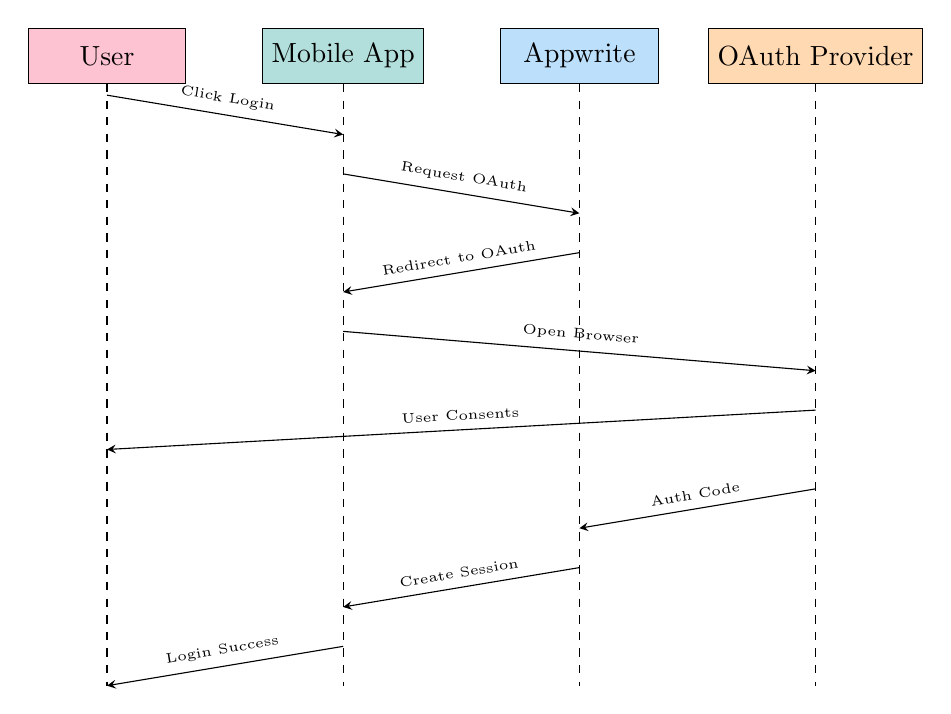
\begin{tikzpicture}[
    node distance=1.2cm,
    entity/.style={rectangle, minimum width=2cm, minimum height=0.7cm, text centered, draw=black, fill=blue!20},
    arrow/.style={->, >=stealth}
]

\node[entity, fill=appwritepink!30] (user) at (0,0) {User};
\node[entity, fill=accentteal!30] (app) at (3,0) {Mobile App};
\node[entity, fill=accentblue!30] (appwrite) at (6,0) {Appwrite};
\node[entity, fill=orange!30] (oauth) at (9,0) {OAuth Provider};

\draw[dashed] (user) -- (0,-8);
\draw[dashed] (app) -- (3,-8);
\draw[dashed] (appwrite) -- (6,-8);
\draw[dashed] (oauth) -- (9,-8);

\draw[arrow] (0,-0.5) -- node[above, sloped, font=\tiny] {Click Login} (3,-1);
\draw[arrow] (3,-1.5) -- node[above, sloped, font=\tiny] {Request OAuth} (6,-2);
\draw[arrow] (6,-2.5) -- node[above, sloped, font=\tiny] {Redirect to OAuth} (3,-3);
\draw[arrow] (3,-3.5) -- node[above, sloped, font=\tiny] {Open Browser} (9,-4);
\draw[arrow] (9,-4.5) -- node[above, sloped, font=\tiny] {User Consents} (0,-5);
\draw[arrow] (9,-5.5) -- node[above, sloped, font=\tiny] {Auth Code} (6,-6);
\draw[arrow] (6,-6.5) -- node[above, sloped, font=\tiny] {Create Session} (3,-7);
\draw[arrow] (3,-7.5) -- node[above, sloped, font=\tiny] {Login Success} (0,-8);

\end{tikzpicture}
\caption{OAuth Authentication Sequence}
\end{figure}

% ============================================
% CHAPTER 4: DATABASES
% ============================================
\chapter{Databases}

\section{Database Overview}

\begin{definitionbox}
Appwrite Databases is a NoSQL document database service that allows you to store and query structured data. It provides a flexible schema with support for relationships, queries, and real-time updates.
\end{definitionbox}

\section{Database Hierarchy}

\begin{figure}[h]
\centering
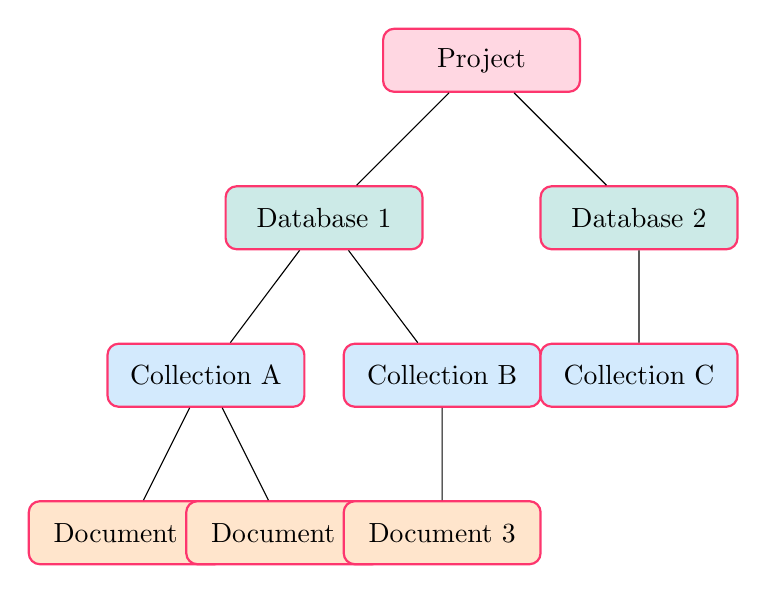
\begin{tikzpicture}[
    level 1/.style={sibling distance=4cm, level distance=2cm},
    level 2/.style={sibling distance=3cm, level distance=2cm},
    level 3/.style={sibling distance=2cm, level distance=2cm},
    box/.style={rectangle, rounded corners, draw=appwritepink, thick, fill=appwritepink!20, minimum width=2.5cm, minimum height=0.8cm}
]

\node[box] {Project}
    child {node[box, fill=accentteal!20] {Database 1}
        child {node[box, fill=accentblue!20] {Collection A}
            child {node[box, fill=orange!20] {Document 1}}
            child {node[box, fill=orange!20] {Document 2}}
        }
        child {node[box, fill=accentblue!20] {Collection B}
            child {node[box, fill=orange!20] {Document 3}}
        }
    }
    child {node[box, fill=accentteal!20] {Database 2}
        child {node[box, fill=accentblue!20] {Collection C}}
    };

\end{tikzpicture}
\caption{Database Hierarchy Structure}
\end{figure}

\section{Data Types}

\begin{table}[h]
\centering
\begin{tabularx}{\textwidth}{l X l}
\toprule
\textbf{Type} & \textbf{Description} & \textbf{Example} \\
\midrule
String & Text data & "John Doe" \\
Integer & Whole numbers & 42 \\
Float & Decimal numbers & 3.14159 \\
Boolean & True/False values & true \\
DateTime & Date and time & 2024-12-17T10:00:00 \\
Email & Email addresses & user@example.com \\
URL & Web addresses & https://example.com \\
IP Address & IP addresses & 192.168.1.1 \\
Enum & Predefined values & ["active", "pending"] \\
Relationship & Link to other documents & Document ID \\
\bottomrule
\end{tabularx}
\caption{Supported Data Types}
\end{table}

\section{CRUD Operations}

\subsection{Create Document}

\begin{lstlisting}[language=JavaScript, caption=Creating a Document]
import { Client, Databases, ID } from "appwrite";

const databases = new Databases(client);

const document = await databases.createDocument(
    'DATABASE_ID',
    'COLLECTION_ID',
    ID.unique(),
    {
        name: 'Luxury Villa',
        price: 500000,
        bedrooms: 4,
        available: true
    }
);
\end{lstlisting}

\subsection{Read Documents}

\begin{lstlisting}[language=JavaScript, caption=Querying Documents]
import { Query } from "appwrite";

// Get all documents
const documents = await databases.listDocuments(
    'DATABASE_ID',
    'COLLECTION_ID'
);

// Query with filters
const filtered = await databases.listDocuments(
    'DATABASE_ID',
    'COLLECTION_ID',
    [
        Query.equal('available', true),
        Query.greaterThan('price', 100000),
        Query.orderDesc('price'),
        Query.limit(10)
    ]
);
\end{lstlisting}

\subsection{Update Document}

\begin{lstlisting}[language=JavaScript, caption=Updating a Document]
const updated = await databases.updateDocument(
    'DATABASE_ID',
    'COLLECTION_ID',
    'DOCUMENT_ID',
    {
        price: 450000,
        available: false
    }
);
\end{lstlisting}

\subsection{Delete Document}

\begin{lstlisting}[language=JavaScript, caption=Deleting a Document]
await databases.deleteDocument(
    'DATABASE_ID',
    'COLLECTION_ID',
    'DOCUMENT_ID'
);
\end{lstlisting}

\section{Queries and Filters}

\begin{table}[h]
\small
\centering
\begin{tabularx}{\textwidth}{l X}
\toprule
\textbf{Query Method} & \textbf{Description} \\
\midrule
Query.equal() & Match exact value \\
Query.notEqual() & Don't match value \\
Query.lessThan() & Less than value \\
Query.greaterThan() & Greater than value \\
Query.search() & Full-text search \\
Query.orderAsc() & Sort ascending \\
Query.orderDesc() & Sort descending \\
Query.limit() & Limit results \\
Query.offset() & Skip results \\
Query.cursorAfter() & Pagination cursor \\
\bottomrule
\end{tabularx}
\caption{Query Methods}
\end{table}

\section{Relationships}

Appwrite supports three types of relationships:

\begin{enumerate}
    \item \textbf{One-to-One} - Single document relates to single document
    \item \textbf{One-to-Many} - Single document relates to multiple documents
    \item \textbf{Many-to-Many} - Multiple documents relate to multiple documents
\end{enumerate}

\begin{lstlisting}[language=JavaScript, caption=Using Relationships]
// Create a property with agent relationship
const property = await databases.createDocument(
    'DATABASE_ID',
    'PROPERTIES',
    ID.unique(),
    {
        name: 'Modern Apartment',
        agent: 'AGENT_DOCUMENT_ID',  // Relationship
        reviews: ['REVIEW_1', 'REVIEW_2']  // Multiple relationships
    }
);

// Fetch with related data
const propertyWithAgent = await databases.getDocument(
    'DATABASE_ID',
    'PROPERTIES',
    'PROPERTY_ID'
);
// Agent data is automatically included
\end{lstlisting}

% ============================================
% CHAPTER 5: STORAGE
% ============================================
\chapter{Storage \& File Management}

\section{Storage Overview}

\begin{keypoint}
Appwrite Storage provides secure file storage with built-in CDN, image manipulation, and virus scanning. Perfect for storing user uploads, images, videos, and documents.
\end{keypoint}

\section{Storage Features}

\begin{itemize}
    \item \textbf{File Upload} - Support for files up to 5GB
    \item \textbf{Image Manipulation} - Resize, crop, compress on-the-fly
    \item \textbf{Virus Scanning} - ClamAV integration
    \item \textbf{File Preview} - Generate thumbnails
    \item \textbf{CDN Integration} - Fast global delivery
    \item \textbf{Compression} - Automatic file compression
\end{itemize}

\section{File Operations}

\subsection{Upload File}

\begin{lstlisting}[language=JavaScript, caption=Uploading a File]
import { Storage, ID } from "appwrite";

const storage = new Storage(client);

// Upload file
const file = await storage.createFile(
    'BUCKET_ID',
    ID.unique(),
    document.getElementById('file-input').files[0],
    ['read("any")']  // Permissions
);

console.log('File uploaded:', file.$id);
\end{lstlisting}

\subsection{Get File URL}

\begin{lstlisting}[language=JavaScript, caption=Getting File URL]
// Get file view URL
const url = storage.getFileView('BUCKET_ID', 'FILE_ID');

// Get file download URL
const downloadUrl = storage.getFileDownload('BUCKET_ID', 'FILE_ID');

// Get file preview with manipulation
const preview = storage.getFilePreview(
    'BUCKET_ID',
    'FILE_ID',
    400,    // width
    300,    // height
    'center', // gravity
    90,     // quality
    0,      // border width
    'FFFFFF', // border color
    0,      // border radius
    1,      // opacity
    0,      // rotation
    'FFFFFF', // background
    'webp'  // output format
);
\end{lstlisting}

\subsection{Delete File}

\begin{lstlisting}[language=JavaScript, caption=Deleting a File]
await storage.deleteFile('BUCKET_ID', 'FILE_ID');
\end{lstlisting}

\section{Image Manipulation}

\begin{table}[h]
\centering
\begin{tabularx}{\textwidth}{l X l}
\toprule
\textbf{Parameter} & \textbf{Description} & \textbf{Values} \\
\midrule
width & Image width in pixels & 0-4000 \\
height & Image height in pixels & 0-4000 \\
gravity & Crop position & center, top, bottom, etc. \\
quality & Image quality & 0-100 \\
borderWidth & Border width & 0-100 \\
borderRadius & Corner radius & 0-4000 \\
output & Output format & jpg, png, gif, webp \\
\bottomrule
\end{tabularx}
\caption{Image Manipulation Parameters}
\end{table}

% ============================================
% CHAPTER 6: CLOUD FUNCTIONS
% ============================================
\chapter{Cloud Functions}

\section{Functions Overview}

\begin{definitionbox}
Appwrite Functions are serverless compute solutions that allow you to run custom backend code in response to events or HTTP requests. They execute in isolated Docker containers with support for 15+ programming languages.
\end{definitionbox}

\section{Supported Runtimes}

\begin{multicols}{3}
\begin{itemize}
    \item Node.js
    \item Python
    \item PHP
    \item Ruby
    \item Dart
    \item Deno
    \item Java
    \item Swift
    \item Kotlin
    \item .NET
    \item C++
    \item Go
\end{itemize}
\end{multicols}

\section{Function Triggers}

\begin{table}[h]
\centering
\begin{tabularx}{\textwidth}{l X}
\toprule
\textbf{Trigger Type} & \textbf{Description} \\
\midrule
HTTP & Execute via HTTP request \\
Event & Trigger on database/storage/auth events \\
Schedule & Run on cron schedule \\
\bottomrule
\end{tabularx}
\caption{Function Trigger Types}
\end{table}

\section{Function Example}

\begin{lstlisting}[language=JavaScript, caption=Node.js Function Example]
// Send welcome email when user registers
export default async ({ req, res, log, error }) => {
    const userId = req.body.userId;
    const email = req.body.email;
    
    try {
        // Send welcome email logic
        log(`Sending welcome email to ${email}`);
        
        // Your email sending code here
        
        return res.json({
            success: true,
            message: 'Welcome email sent'
        });
    } catch (err) {
        error('Failed to send email: ' + err.message);
        return res.json({
            success: false,
            error: err.message
        }, 500);
    }
};
\end{lstlisting}

\section{Use Cases}

\begin{enumerate}
    \item \textbf{Payment Processing} - Handle Stripe/PayPal webhooks
    \item \textbf{Email Notifications} - Send transactional emails
    \item \textbf{Data Processing} - Process uploaded files
    \item \textbf{Third-Party Integration} - Connect to external APIs
    \item \textbf{Scheduled Tasks} - Database cleanup, reports
    \item \textbf{Custom Business Logic} - Complex calculations
\end{enumerate}

% ============================================
% CHAPTER 7: REALTIME
% ============================================
\chapter{Realtime}

\section{Realtime Overview}

\begin{keypoint}
Appwrite Realtime enables WebSocket connections to subscribe to events and receive live updates when data changes. Perfect for chat apps, notifications, and collaborative features.
\end{keypoint}

\section{Realtime Implementation}

\begin{lstlisting}[language=JavaScript, caption=Subscribe to Realtime Events]
import { Client } from "appwrite";

const client = new Client()
    .setEndpoint('https://cloud.appwrite.io/v1')
    .setProject('YOUR_PROJECT_ID');

// Subscribe to document updates
client.subscribe('databases.DATABASE_ID.collections.COLLECTION_ID.documents', response => {
    console.log('Event:', response.events);
    console.log('Payload:', response.payload);
});

// Subscribe to specific document
client.subscribe('databases.DATABASE_ID.collections.COLLECTION_ID.documents.DOCUMENT_ID', response => {
    console.log('Document updated:', response.payload);
});

// Subscribe to account events
client.subscribe('account', response => {
    console.log('Account event:', response);
});
\end{lstlisting}

\section{Event Types}

\begin{table}[h]
\centering
\begin{tabularx}{\textwidth}{l X}
\toprule
\textbf{Event} & \textbf{Description} \\
\midrule
*.create & Document/file created \\
*.update & Document/file updated \\
*.delete & Document/file deleted \\
account.* & Account events \\
databases.*.* & Database events \\
storage.*.* & Storage events \\
functions.*.* & Function execution events \\
\bottomrule
\end{tabularx}
\caption{Realtime Event Types}
\end{table}

% ============================================
% CHAPTER 8: PERMISSIONS & SECURITY
% ============================================
\chapter{Permissions \& Security}

\section{Permission System}

Appwrite uses a role-based permission system for fine-grained access control.

\section{Permission Roles}

\begin{table}[h]
\centering
\begin{tabularx}{\textwidth}{l X}
\toprule
\textbf{Role} & \textbf{Description} \\
\midrule
any() & Anyone (authenticated or guest) \\
guests() & Unauthenticated users \\
users() & Any authenticated user \\
user(ID) & Specific user by ID \\
team(ID) & All team members \\
member(ID) & Specific team member \\
\bottomrule
\end{tabularx}
\caption{Permission Roles}
\end{table}

\section{Permission Types}

\begin{itemize}
    \item \textbf{Read} - View documents/files
    \item \textbf{Create} - Create new documents/files
    \item \textbf{Update} - Modify existing documents/files
    \item \textbf{Delete} - Remove documents/files
\end{itemize}

\section{Setting Permissions}

\begin{lstlisting}[language=JavaScript, caption=Permission Examples]
import { Permission, Role } from "appwrite";

// Create document with permissions
const document = await databases.createDocument(
    'DATABASE_ID',
    'COLLECTION_ID',
    ID.unique(),
    { title: 'My Document' },
    [
        Permission.read(Role.any()),
        Permission.update(Role.user('USER_ID')),
        Permission.delete(Role.user('USER_ID'))
    ]
);

// File with team permissions
const file = await storage.createFile(
    'BUCKET_ID',
    ID.unique(),
    fileInput.files[0],
    [
        Permission.read(Role.team('TEAM_ID')),
        Permission.delete(Role.team('TEAM_ID', 'owner'))
    ]
);
\end{lstlisting}

% ============================================
% CHAPTER 9: SETUP GUIDE
% ============================================
\chapter{Setup \& Configuration}

\section{Creating an Appwrite Account}

\begin{enumerate}
    \item Visit \url{https://cloud.appwrite.io}
    \item Click "Sign Up" or "Get Started"
    \item Choose sign-up method (Email, GitHub, etc.)
    \item Verify your email address
    \item Complete your profile
\end{enumerate}

\section{Creating a Project}

\begin{enumerate}
    \item Log in to Appwrite Console
    \item Click "Create Project"
    \item Enter project name
    \item Click "Create"
    \item Note your Project ID
\end{enumerate}

\section{Platform Configuration}

\subsection{iOS Configuration}

\begin{lstlisting}[language=bash, caption=iOS Setup]
# Add bundle identifier
Bundle ID: com.yourcompany.yourapp
Name: Your App Name
\end{lstlisting}

\subsection{Android Configuration}

\begin{lstlisting}[language=bash, caption=Android Setup]
# Add package name
Package Name: com.yourcompany.yourapp
Name: Your App Name
\end{lstlisting}

\section{SDK Installation}

\subsection{React Native}

\begin{lstlisting}[language=bash, caption=Install Appwrite SDK]
npm install appwrite
# or
yarn add appwrite
\end{lstlisting}

\subsection{Flutter}

\begin{lstlisting}[language=bash, caption=Flutter Installation]
flutter pub add appwrite
\end{lstlisting}

\section{SDK Initialization}

\begin{lstlisting}[language=JavaScript, caption=Initialize Appwrite Client]
import { Client, Account, Databases, Storage } from 'appwrite';

const client = new Client();

client
    .setEndpoint('https://cloud.appwrite.io/v1')
    .setProject('YOUR_PROJECT_ID');

const account = new Account(client);
const databases = new Databases(client);
const storage = new Storage(client);

export { client, account, databases, storage };
\end{lstlisting}

% ============================================
% CHAPTER 10: BEST PRACTICES
% ============================================
\chapter{Best Practices}

\section{Security Best Practices}

\begin{enumerate}
    \item \textbf{Use Environment Variables} - Never hardcode API keys
    \item \textbf{Implement Proper Permissions} - Use least privilege principle
    \item \textbf{Enable 2FA} - For admin accounts
    \item \textbf{Regular Audits} - Review access logs
    \item \textbf{HTTPS Only} - Always use secure connections
\end{enumerate}

\section{Performance Optimization}

\begin{itemize}
    \item \textbf{Use Queries Efficiently} - Add indexes for frequently queried fields
    \item \textbf{Implement Pagination} - Use limit and offset
    \item \textbf{Cache Static Data} - Reduce unnecessary API calls
    \item \textbf{Optimize Images} - Use proper dimensions and formats
    \item \textbf{Batch Operations} - Group multiple operations when possible
\end{itemize}

\section{Database Design}

\begin{notebox}
\textbf{Schema Design Tips:}
\begin{itemize}
    \item Keep documents focused and minimal
    \item Use relationships appropriately
    \item Create indexes for search fields
    \item Plan for scalability from the start
    \item Document your schema
\end{itemize}
\end{notebox}

% ============================================
% CHAPTER 11: USE CASES
% ============================================
\chapter{Real-World Use Cases}

\section{Mobile Application Types}

\begin{table}[h]
\centering
\begin{tabularx}{\textwidth}{l X}
\toprule
\textbf{App Type} & \textbf{Appwrite Features Used} \\
\midrule
Social Media & Auth, Database, Storage, Realtime \\
E-Commerce & Auth, Database, Storage, Functions \\
Chat Application & Auth, Database, Realtime \\
Task Management & Auth, Database, Realtime \\
Food Delivery & Auth, Database, Storage, Functions, Realtime \\
Real Estate & Auth, Database, Storage, OAuth \\
Education Platform & Auth, Database, Storage, Functions \\
\bottomrule
\end{tabularx}
\caption{Application Types and Features}
\end{table}

\section{Example: Real Estate App}

\begin{lstlisting}[language=JavaScript, caption=Complete Real Estate Implementation]
// 1. Setup Collections
// Properties: name, type, price, bedrooms, bathrooms, agent
// Agents: name, email, phone, avatar
// Reviews: rating, comment, property, user

// 2. Authentication
const login = async () => {
    await account.createOAuth2Session(
        OAuthProvider.Google,
        successUrl,
        failureUrl
    );
};

// 3. Fetch Properties
const getProperties = async (type) => {
    return await databases.listDocuments(
        'DATABASE_ID',
        'PROPERTIES',
        type ? [Query.equal('type', type)] : []
    );
};

// 4. Upload Property Image
const uploadImage = async (file) => {
    return await storage.createFile(
        'BUCKET_ID',
        ID.unique(),
        file
    );
};

// 5. Subscribe to New Properties
client.subscribe('databases.*.collections.PROPERTIES.documents', 
    response => {
        if (response.events.includes('create')) {
            showNotification('New property available!');
        }
    }
);
\end{lstlisting}

% ============================================
% CHAPTER 12: TROUBLESHOOTING
% ============================================
\chapter{Troubleshooting}

\section{Common Issues}

\subsection{Authentication Errors}

\begin{warningbox}
\textbf{401 Unauthorized}
\begin{itemize}
    \item Check if OAuth provider is enabled in console
    \item Verify redirect URLs are correctly configured
    \item Ensure session is valid
\end{itemize}
\end{warningbox}

\subsection{Database Errors}

\begin{warningbox}
\textbf{Document Not Found}
\begin{itemize}
    \item Verify document ID is correct
    \item Check read permissions
    \item Ensure collection exists
\end{itemize}
\end{warningbox}

\subsection{Storage Errors}

\begin{warningbox}
\textbf{File Upload Failed}
\begin{itemize}
    \item Check file size (max 5GB)
    \item Verify bucket permissions
    \item Ensure valid file type
\end{itemize}
\end{warningbox}

\section{Debug Tips}

\begin{enumerate}
    \item \textbf{Enable Console Logging} - Monitor API requests
    \item \textbf{Check Network Tab} - View request/response
    \item \textbf{Review Logs} - Check Appwrite console logs
    \item \textbf{Test Permissions} - Use console to test access
    \item \textbf{Validate Data} - Ensure proper data structure
\end{enumerate}

% ============================================
% CHAPTER 13: ADVANCED TOPICS
% ============================================
\chapter{Advanced Topics}

\section{Self-Hosting Appwrite}

\begin{lstlisting}[language=bash, caption=Self-Host with Docker]
# Install Appwrite
docker run -it --rm \
    --volume /var/run/docker.sock:/var/run/docker.sock \
    --volume "$(pwd)"/appwrite:/usr/src/code/appwrite:rw \
    --entrypoint="install" \
    appwrite/appwrite:1.4.0

# Start Appwrite
docker compose up -d
\end{lstlisting}

\section{Webhooks}

Configure webhooks to receive HTTP callbacks when events occur:

\begin{lstlisting}[language=JavaScript, caption=Webhook Payload Example]
{
    "events": ["databases.*.collections.*.documents.*.create"],
    "userId": "user123",
    "payload": {
        "$id": "doc123",
        "name": "New Property",
        "price": 250000
    }
}
\end{lstlisting}

\section{Custom Domains}

Set up custom domains for your Appwrite instance:

\begin{enumerate}
    \item Configure DNS records
    \item Add domain in Appwrite console
    \item Enable SSL certificate
    \item Update SDK endpoint
\end{enumerate}

% ============================================
% CONCLUSION
% ============================================
\chapter{Conclusion}

\section{Summary}

Appwrite is a comprehensive Backend-as-a-Service platform that simplifies mobile app development by providing:

\begin{itemize}
    \item \textbf{Complete Authentication} - Multiple providers, secure sessions
    \item \textbf{Powerful Databases} - NoSQL with relationships and queries
    \item \textbf{File Storage} - With CDN and image manipulation
    \item \textbf{Cloud Functions} - Serverless compute
    \item \textbf{Realtime Updates} - WebSocket subscriptions
    \item \textbf{Robust Security} - Fine-grained permissions
\end{itemize}

\section{Getting Started}

\begin{keypoint}
Start building your mobile app today:
\begin{enumerate}
    \item Create free account at \url{https://cloud.appwrite.io}
    \item Set up your first project
    \item Install SDK in your mobile app
    \item Build amazing features!
\end{enumerate}
\end{keypoint}

\section{Resources}

\begin{itemize}
    \item Official Documentation: \url{https://appwrite.io/docs}
    \item GitHub Repository: \url{https://github.com/appwrite/appwrite}
    \item Discord Community: \url{https://appwrite.io/discord}
    \item YouTube Tutorials: \url{https://youtube.com/@appwrite}
\end{itemize}

\vspace{2cm}

\begin{center}
\Large\textbf{Happy Building with Appwrite!}

\vspace{0.5cm}

\textit{Build like a team of hundreds.}
\end{center}

\end{document}
